%2.3_1センサーボードについて

\clearpage
\section{センサーボードを使ってみよう}
\subsection{センサーボードって何だろう}

プログラムによって、画面の上でゲームが遊べることがわかりました。
これはちょうどスマートフォンや家庭用ゲーム機でゲームを遊ぶのと似ています。

今回、皆さんが使うRaspberryPiは、ゲームだけでなく明るさや温度などさまざまな情報を調べることのできるセンサーボードを接続することができます。

\begin{figure}[H]
    \begin{center}
        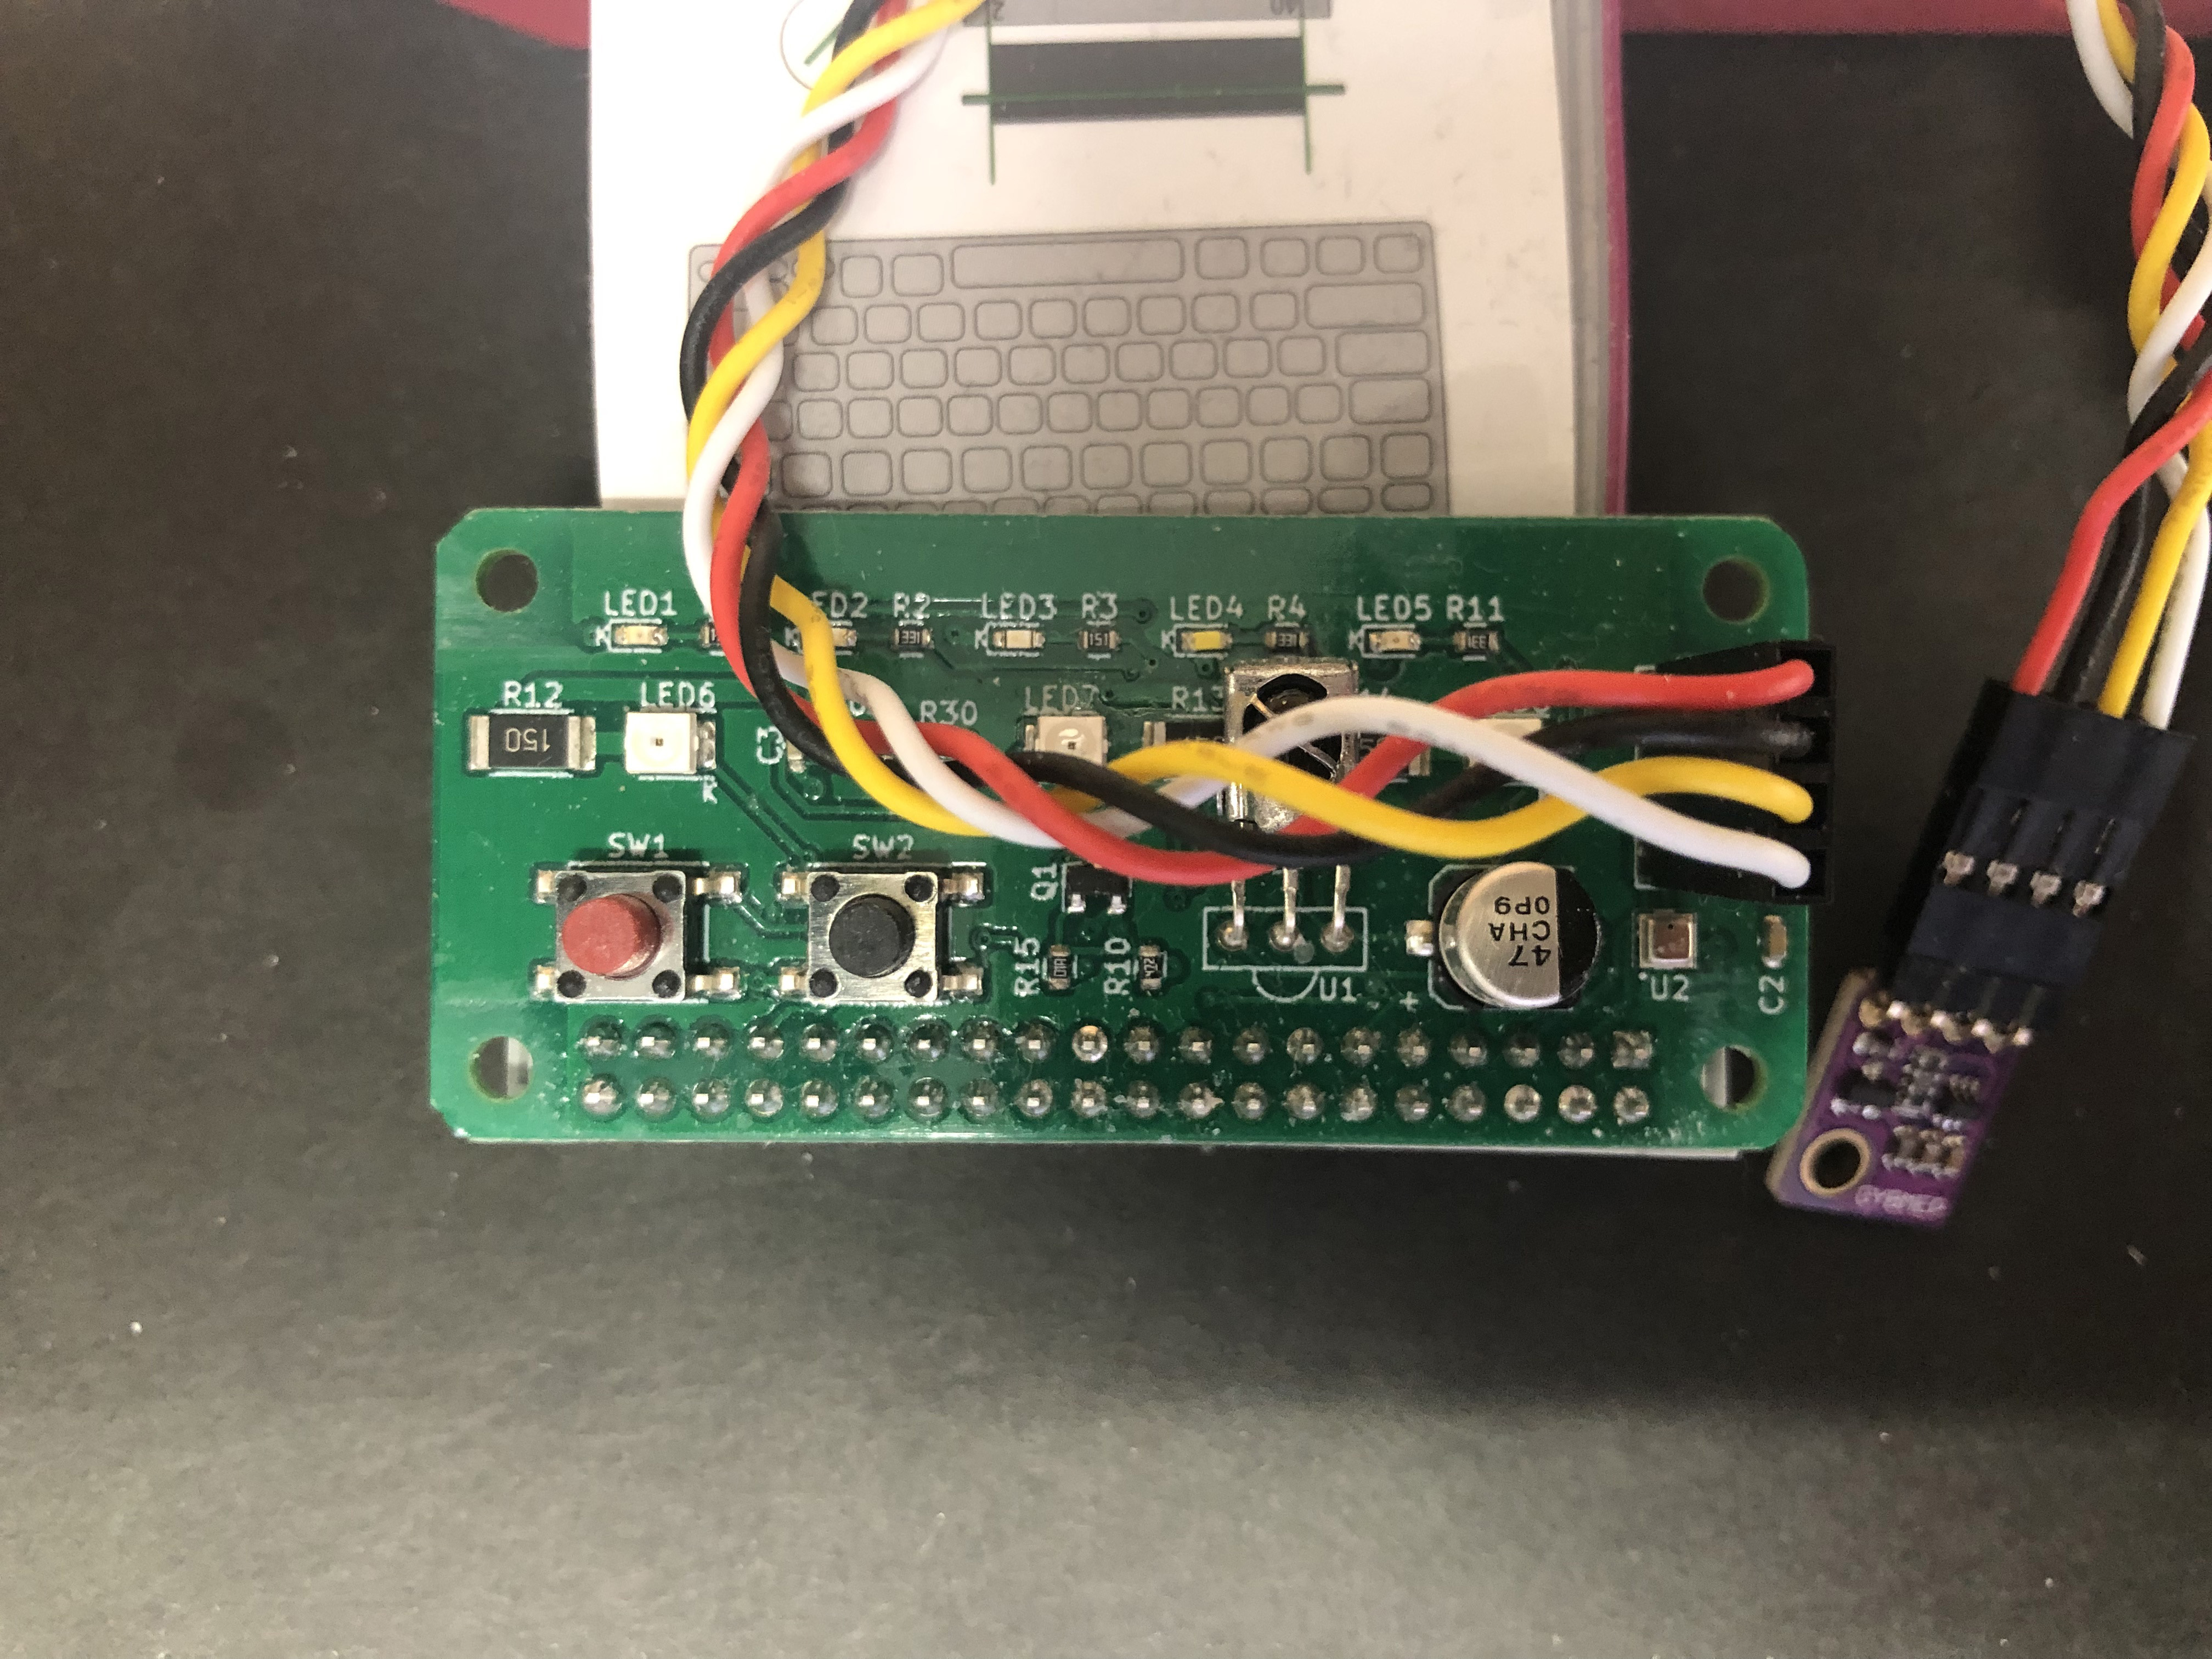
\includegraphics[keepaspectratio,width=9.79cm,height=7.955cm]{text02-img/sensor1.jpg}
        \caption{センサーボード}
    \end{center}
    \label{fig:folder_icon}
\end{figure}

まず最初にRaspberryPiとセンサーボードを接続しましょう。
普通の電気製品は、ケースや保護がありますが、センサーボードやRaspberryPiは、回路の基板そのままの状態です。
触っても感電することはありませんが、静電気によってこわれたりケガをすることがあるので、回路部分を触らないように注意しましょう。

\begin{figure}[H]
    \begin{center}
        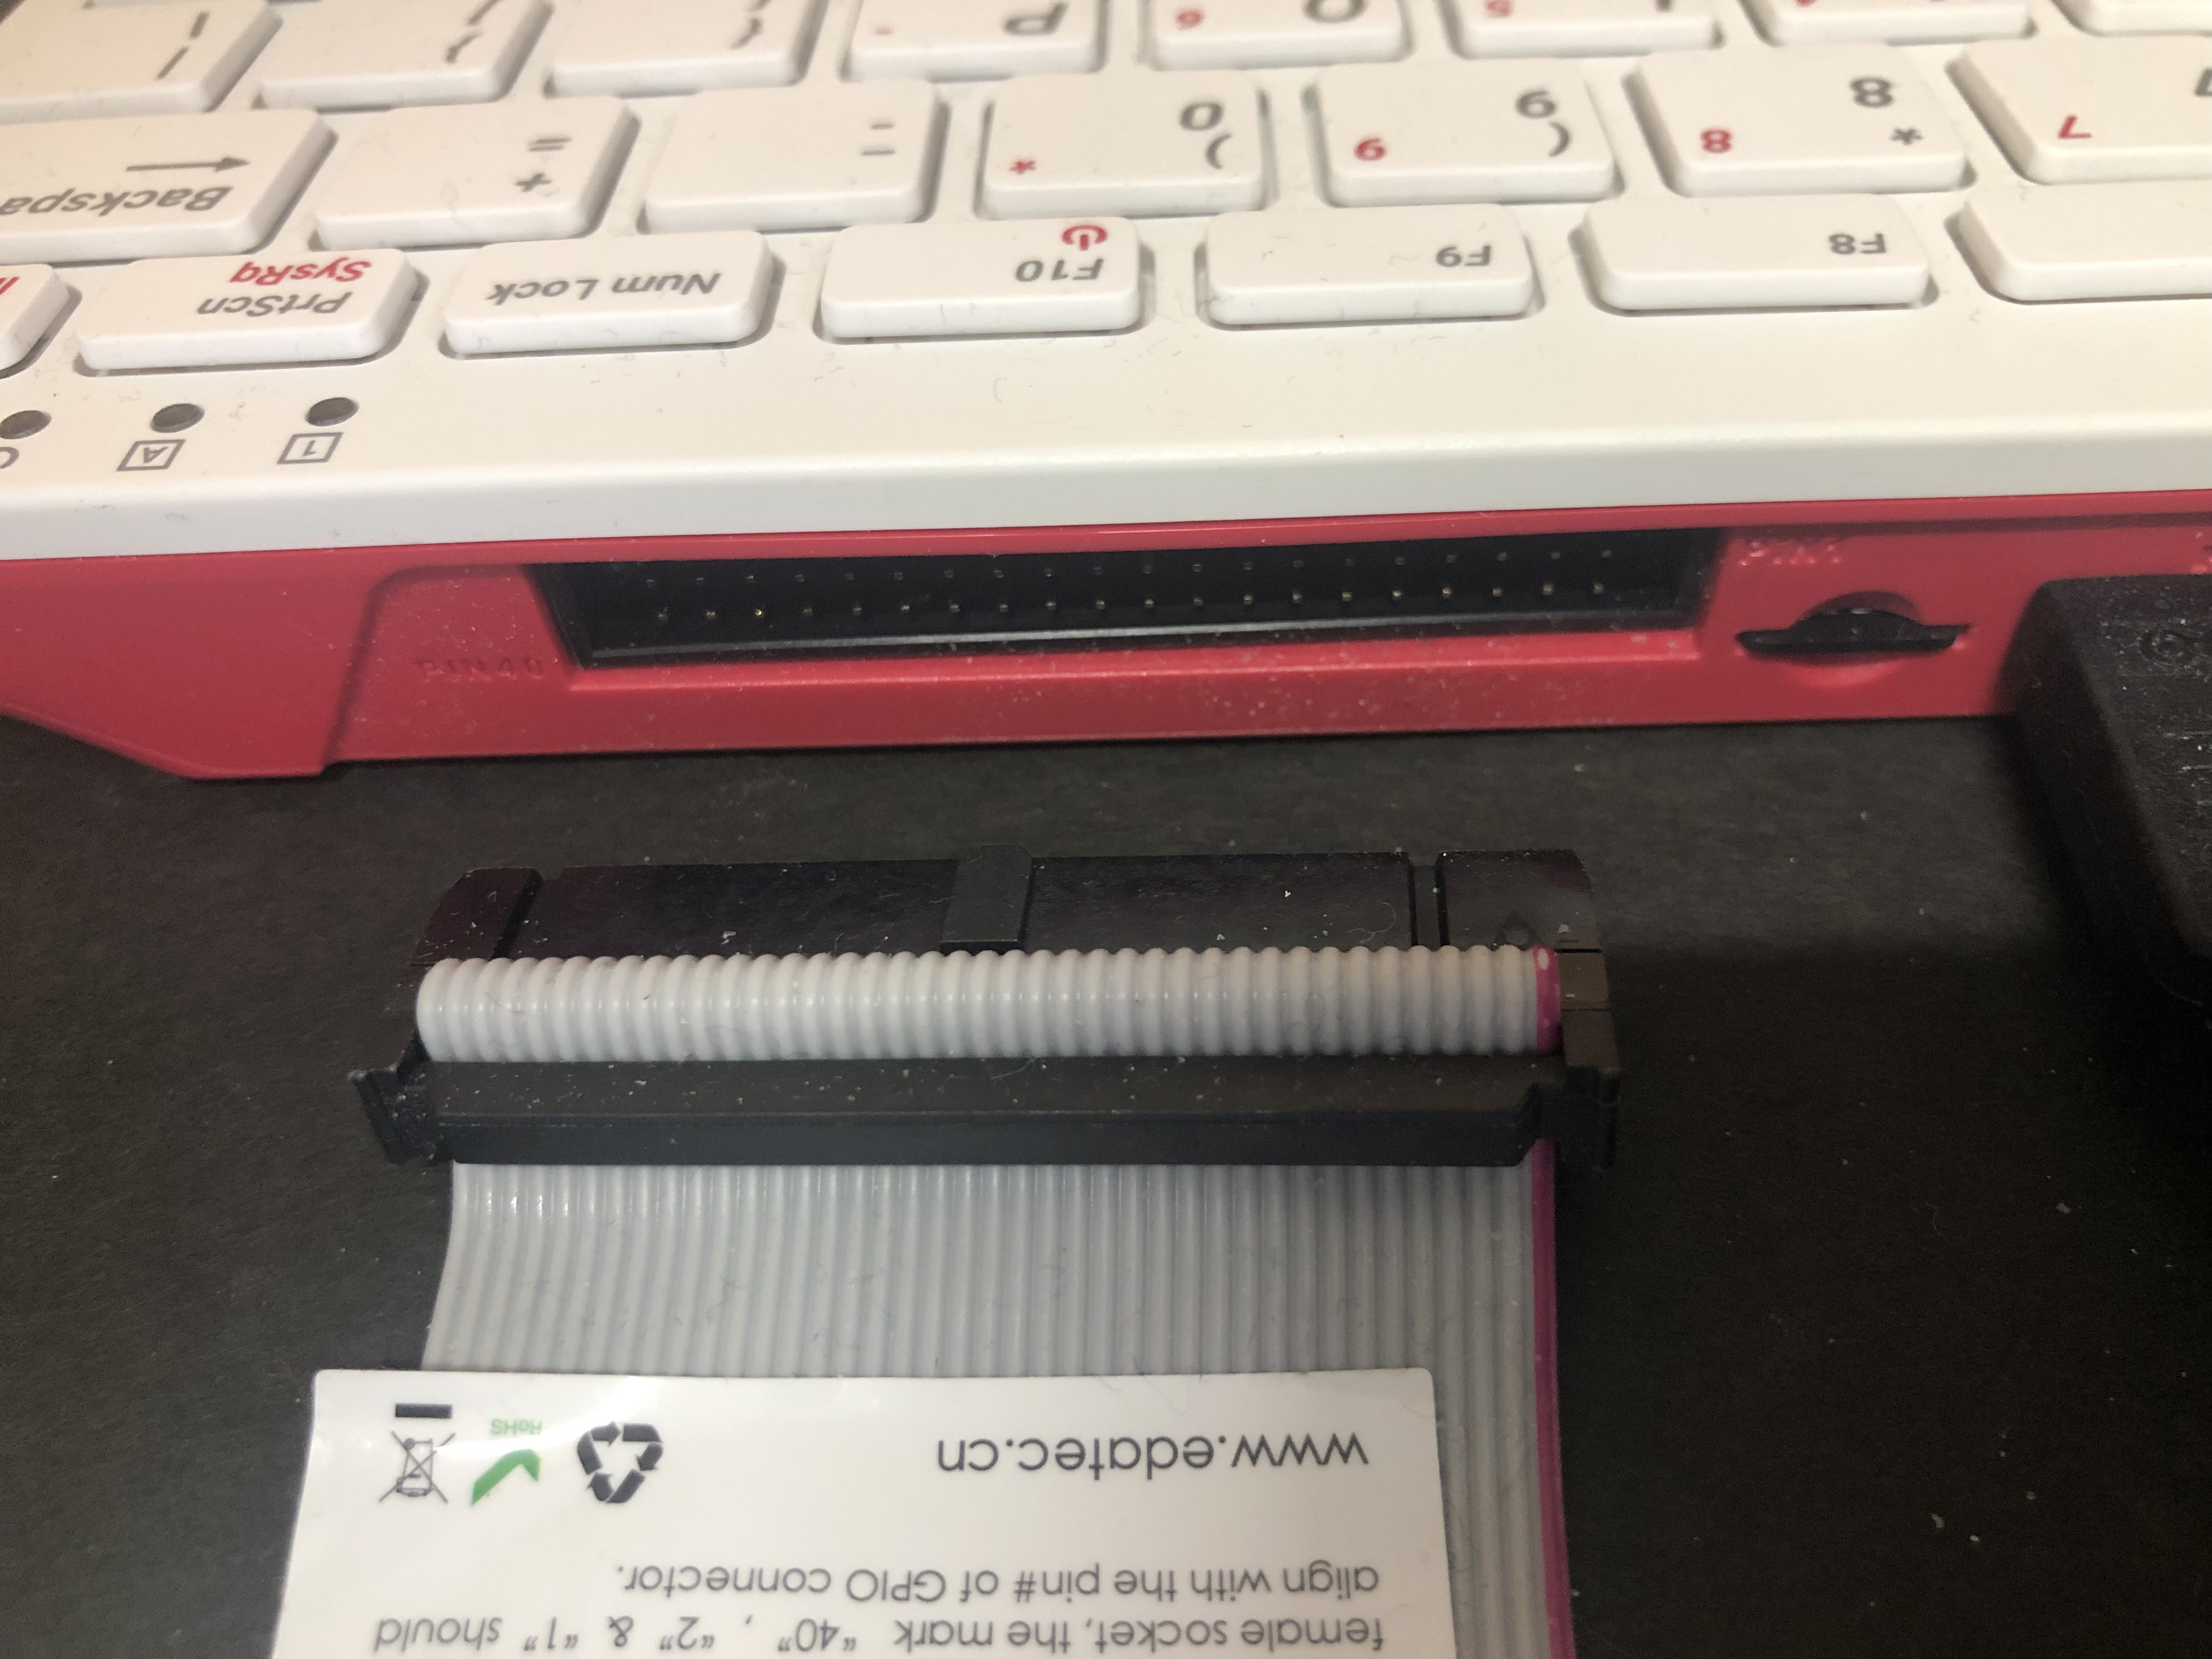
\includegraphics[keepaspectratio,width=9.79cm,height=7.955cm]{text02-img/sensor2.jpg}
        \caption{接続コネクタと拡張ケーブル}
    \end{center}
\end{figure}

RaspberryPiの裏がわに、拡張ケーブルを差し込むための接続コネクタがあるのを確認(かくにん)してください。

拡張ケーブルにセンサーボードをつなげます。ピンの位置がずれたり、さかさまに差さないように注意してください。
正しく差し込まれたことを先生やTAに必ず見てもらってください。

\begin{figure}[H]
    \begin{center}
        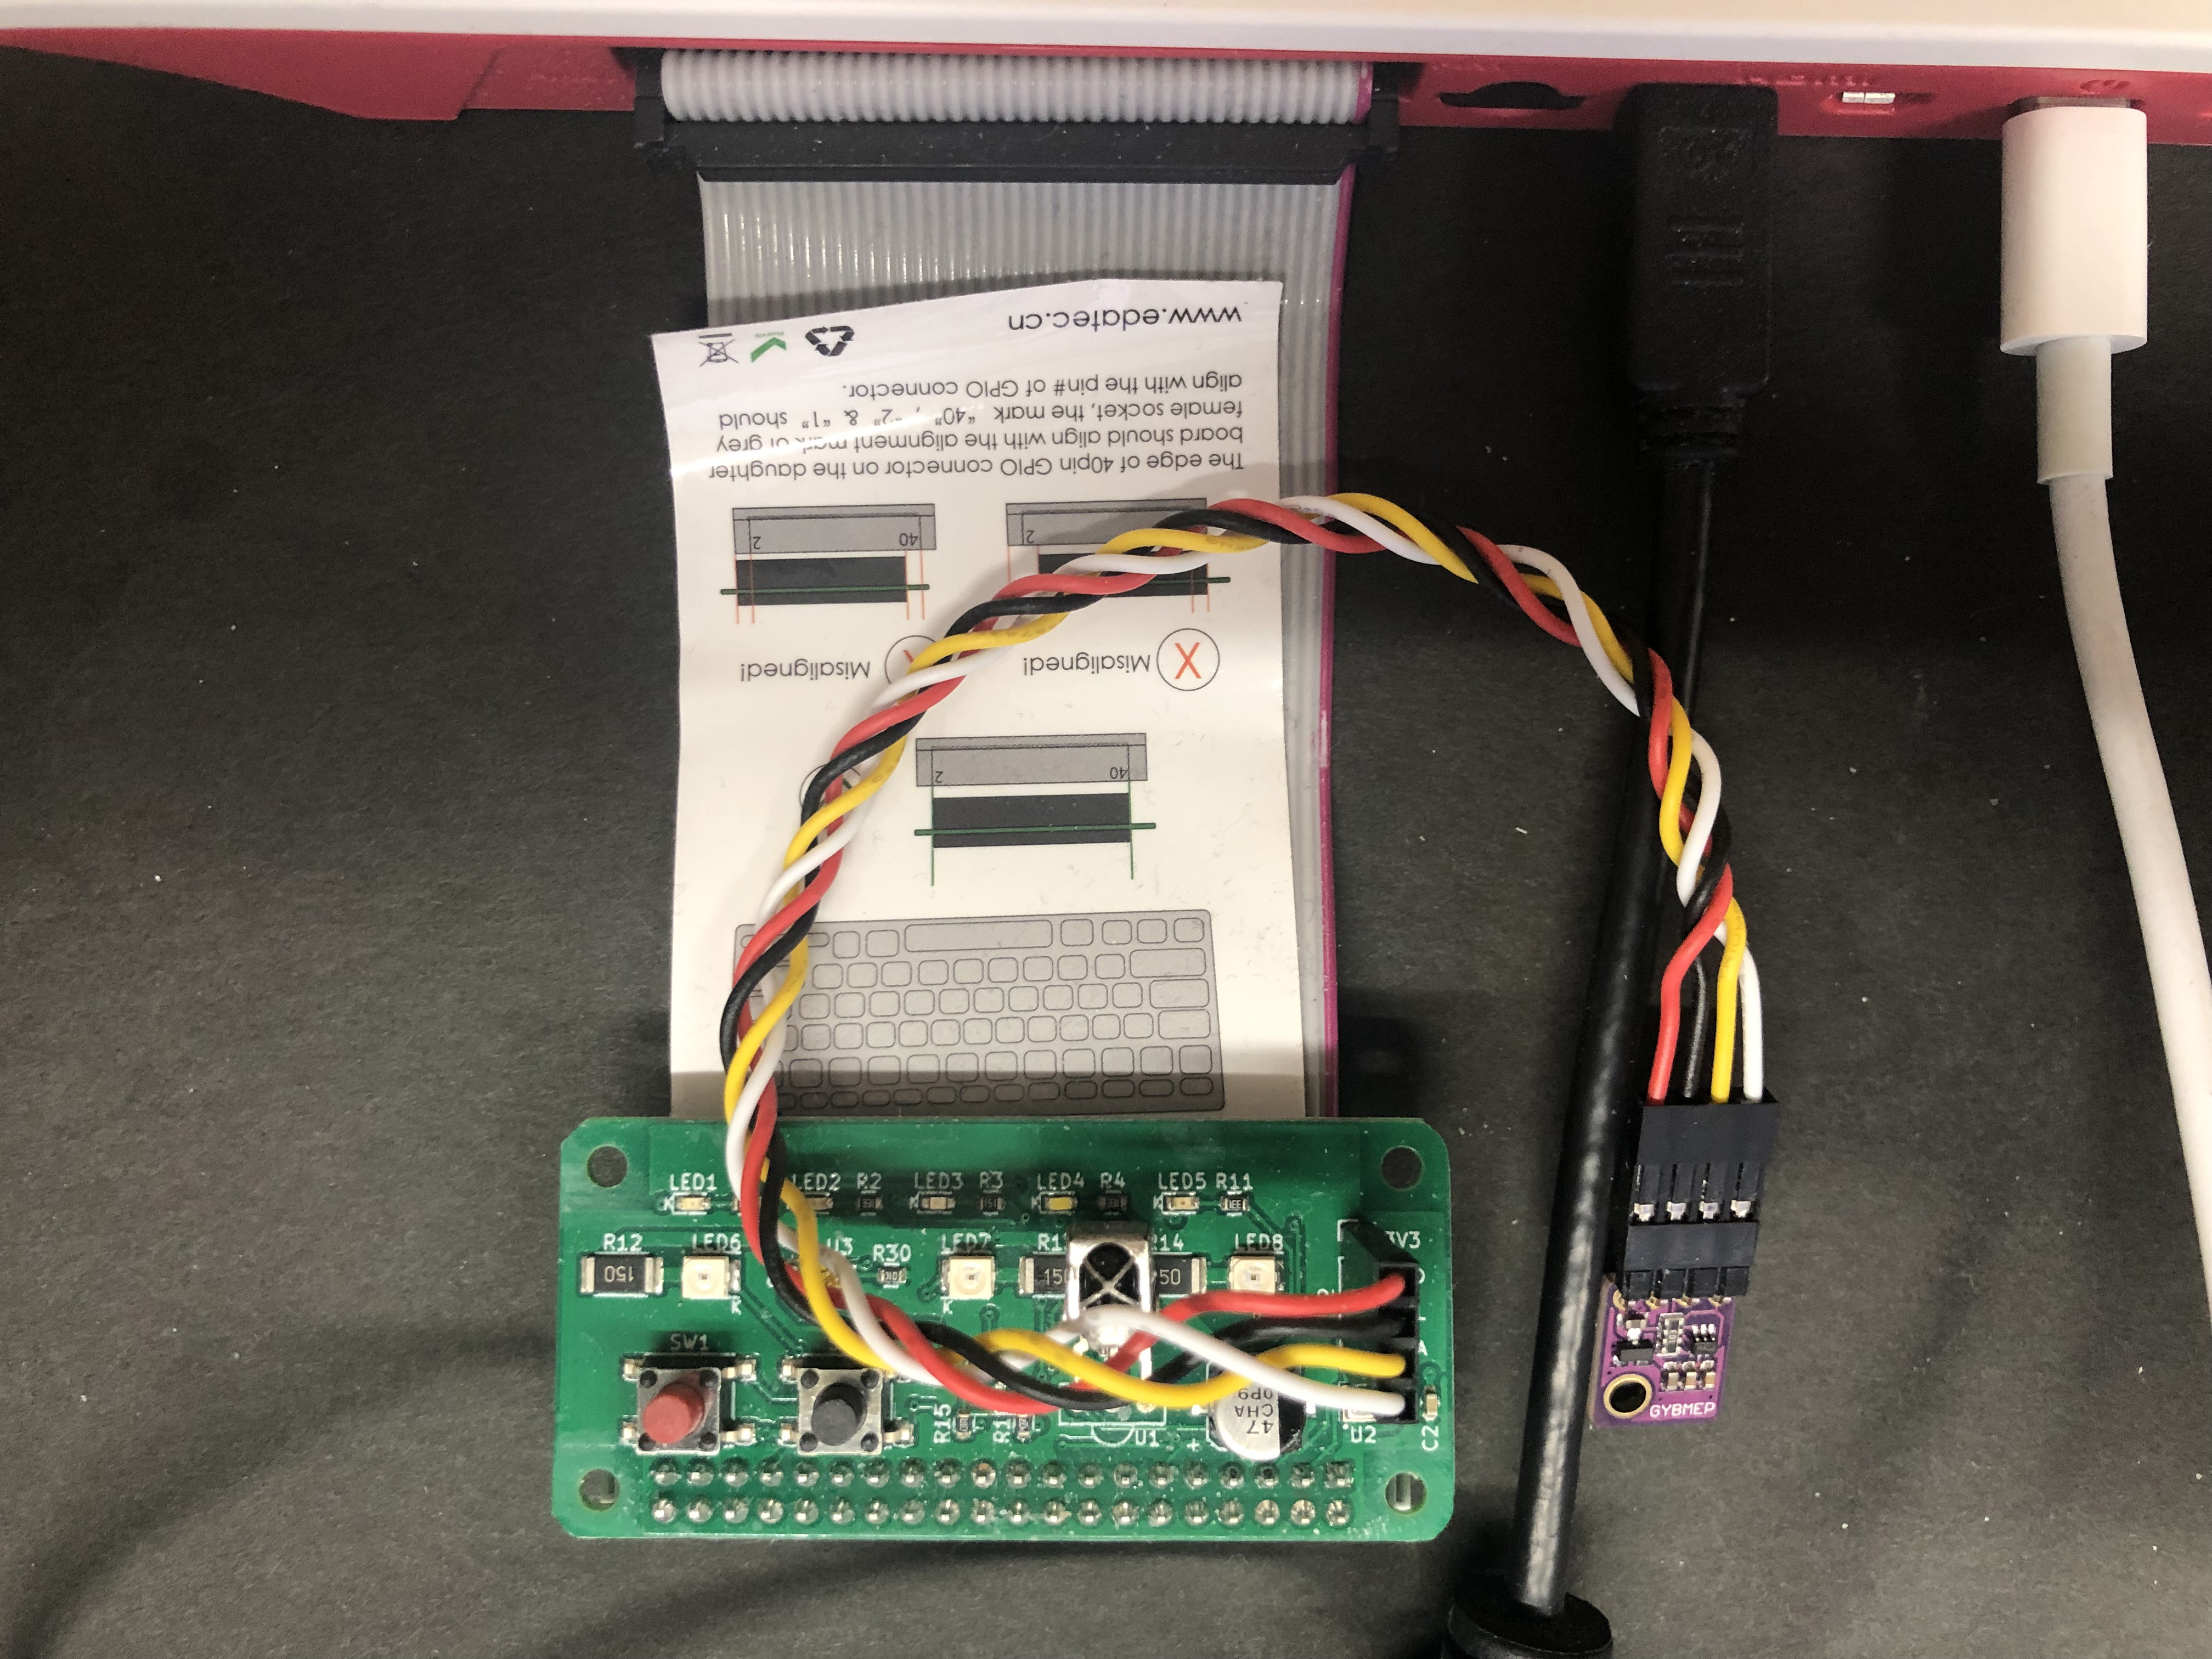
\includegraphics[keepaspectratio,width=9.79cm,height=7.955cm]{text02-img/sensor3.jpg}
        \caption{拡張ケーブルを差し込んだところ}
    \end{center}
\end{figure}

次にRaspberryPi本体に、拡張ケーブルを差し込みます。
きちんと奥まで差し込まれていることを確認(かくにん)しましょう。

\begin{figure}[H]
    \begin{center}
        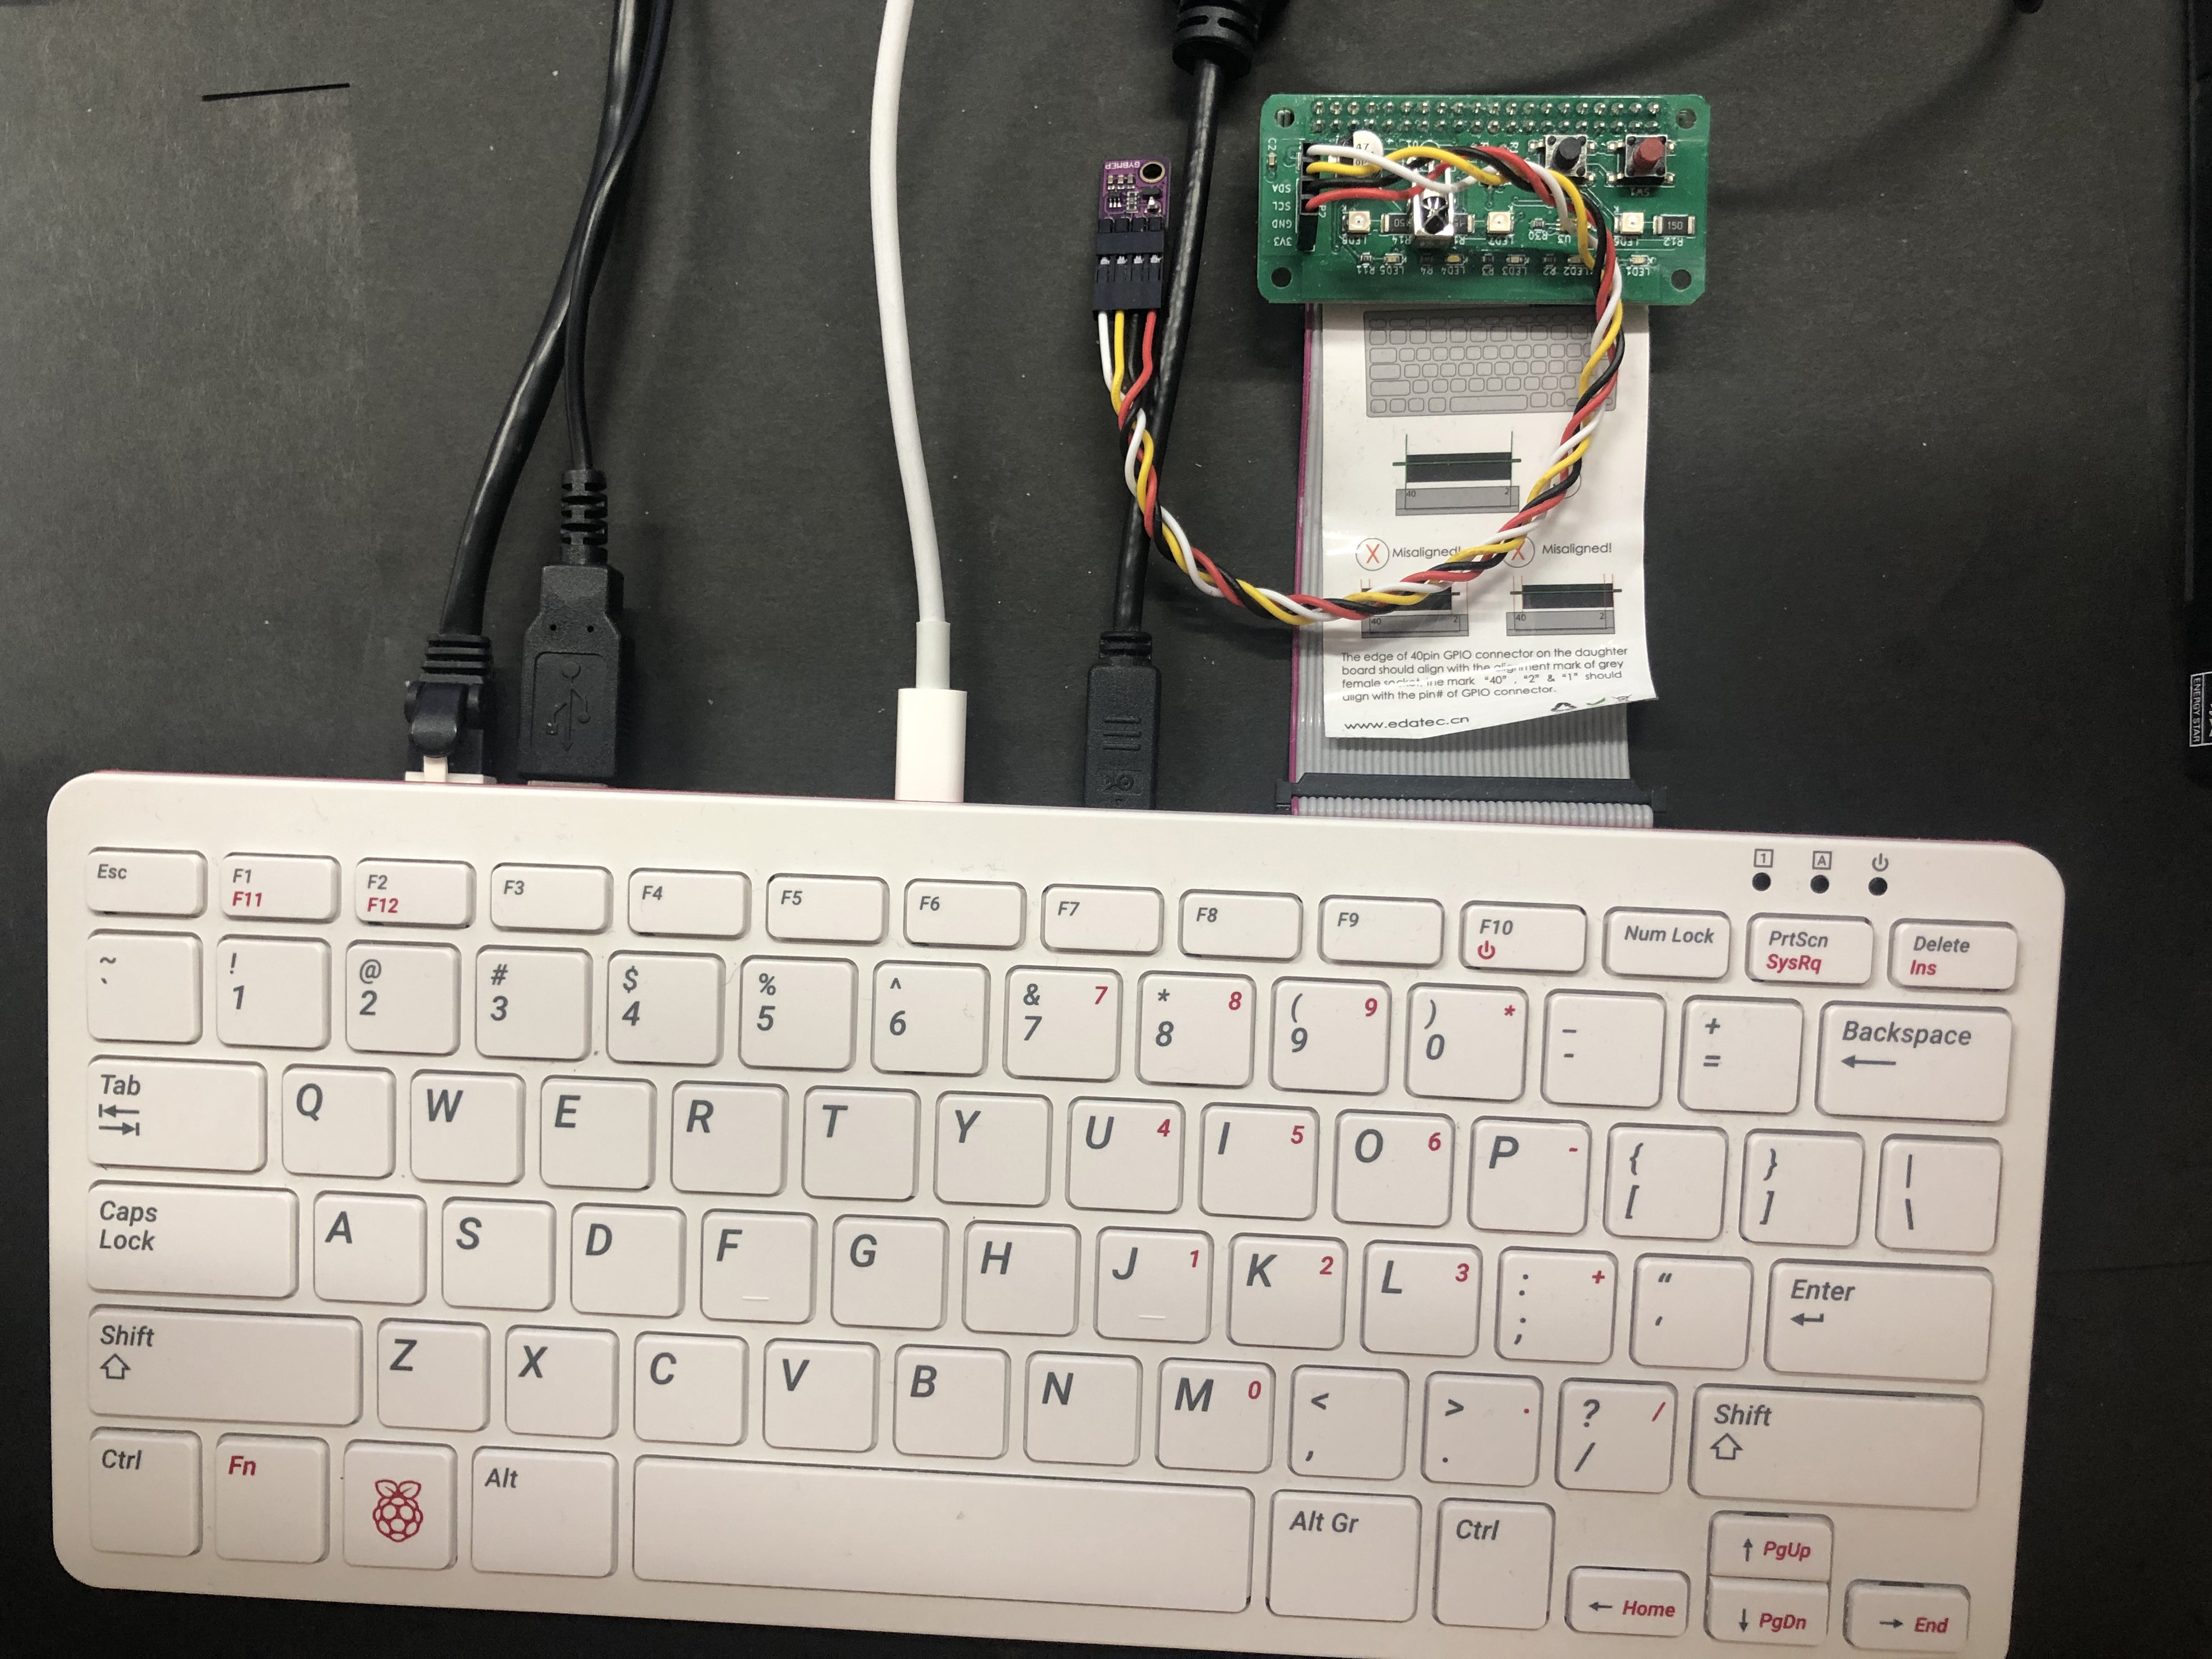
\includegraphics[keepaspectratio,width=9.79cm,height=7.955cm]{text02-img/sensor4.jpg}
        \caption{Raspberry Piとセンサーボード}
    \end{center}
\end{figure}

これで、接続されたセンサーボードを使ったプログラムが動くようになります。
プログラミングは、画面を動かすだけでなく、RaspberryPiが持つすべての機能を自由に組み合わせて使うことができるのです。

それでは、さっそくプログラミングを始めてみましょう。
これから、やることの内容はつぎの通りです。

\begin{itemize}
    \item \textgt{\bf LEDがてんめつするスクリプト(gpio)を読み込んで動かす}
    \item \textgt{\bf メッセージが出るスクリプト(mes)を改造してみる}
    \item \textgt{\bf エディタの編集について覚える}
    \item \textgt{\bf 別なLEDを光らせてみよう}
    \item \textgt{\bf 別なメッセージを出してみよう}
    \item \textgt{\bf 改造したスクリプトを保存してみよう}
    \item \textgt{\bf 命令とパラメーターを覚えよう}
\end{itemize}